% !TeX root = ../thuthesis-example.tex

\chapter{引言}


\section{研究背景}

网络自诞生以来,随着数十年的发展,已经成为了最重要的信息化基础设施之一。如图~\ref{fig:网民规模和互联网普及率}所示,第46次《中国互联网络发展状况统计报告》\cite{cac.gov} 指出,截至2020年6月,我国的移动网民用户规模已经累计达到9.40亿,互联网的网络普及率已经高达67.0\%,互联网的主要应用领域覆盖范围已经达到包括即时移动通信、搜索结果引擎、网络即时新闻、线下线上教育、购物以及出行等各个方面,可以说如今互联网已经和每一个人的工作日常生活息息相关密不可分。



\begin{figure}
    \centering
    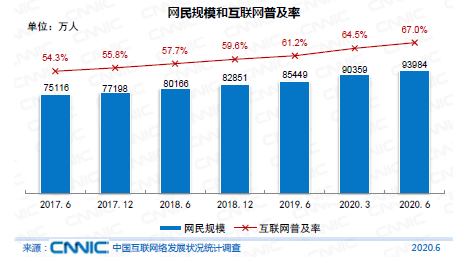
\includegraphics[width=0.6\linewidth]{网民规模.PNG}
    \caption{网民规模和互联网普及率}
    \label{fig:网民规模和互联网普及率}
  \end{figure}

随着网络重要性的提升、用户规模的膨胀,管理网络的难度也越来越大。网络系统就是一个繁琐而又复杂的网络,它的设计、运营以及维护都必须依靠专业的网络运维技术人员。早期的网络运维管理工作绝大多数都是由运维工作人员手工操作来完成,此后人们逐渐发现一些重复性的工作可以用自动化脚本来实现,于是诞生了自动化运维。自动化的运维系统可以认为是一种建立在专家经验和人为制订规则的系统之上。但是随着移动互联网的规模迅速增长和巨大扩展,以及其服务种类和方式的日益多样化,由人们自主设定的基础运维规则当中的方法与技术,渐渐难以应付企业的大规模运维需求。在此情况下,智能运维应运而生。它与自动化运维仰仗专门人员的知识、人为制定规则有别,智能运维的着重点在于使用新颖的机器学习算法,先从庞大的运维管理数据中反复吸收经验进行学习,进而有条不紊的逐步提取规则。

% 随着网络重要性的提升、用户规模的膨胀,管理网络的难度也越来越大。网络是一个复杂的系统,它的部署、运行和维护都需要专业的运维人员。
% 早期的运维工作大部分是由运维人员手工完成,此后人们逐渐发现一些重复性的工作可以用自动化脚本来实现,于是诞生了自动化运维。自动化运维可以被认为是基于专家经验、人为制定规则的系统。
% 但是随着互联网规模急剧膨胀,以及服务类型的多样化,简单的、基于人为制定规则的方法并不能解决大规模运维的问题,因此产生了智能运维。与自动化运维依赖专家知识、人工生成规则不同,
% 智能运维强调使用机器学习算法从海量运维数据中不断学习、不断提炼规则。

异常检测是智能运维的关键环节,具有至关重要的意义。从网络故障管理的角度来说,做好异常检测可以提前预测故障的发生;从性能管理的角度来说,可以发现性能不佳的区域,避免因误配置、架构不合理导致性能下降;
从安全管理的角度来说,在网络攻击的前期阶段,及时发现并预警后续攻击,进而做出防御措施。因此,在复杂的网络环境中甄别出有效和异常流量尤为重要,在重大事故发生前,
根据各项流量特征的变化,提前预测出即将发生的事故,提高应急响应速度,防患于未然。


本文以校园网为例,进行网络流量异常检测算法和系统的研究。清华大学校园网是全球规模最大,架构最复杂,流量场景最多变的校园网之一,具有以下几个特点:
\begin{enumerate}
    \item 用户规模大,流量峰值高。每天有10万台设备活跃在线,同时在线设备最多为7万台,峰值流量约为30Gbps/s,如图~\ref{fig:用户流量变化图}所示。
    \item	用户应用类型多,如图~\ref{fig:用户应用类型图}所示,清华大学校园网中的用户类型远比一般的企业网复杂,在网络环境中几百种应用同时使用,这给数据分析带来了很多困难。
    \item	异常流量是常态。扫描流量、攻击流量占比多。
\end{enumerate}

\begin{figure}
  \centering
  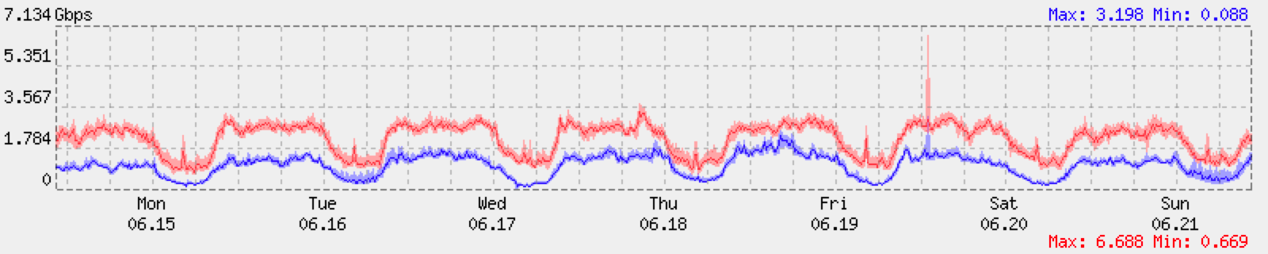
\includegraphics[width=0.6\linewidth]{用户流量变化图.png}
  \caption{用户流量变化图}
  \label{fig:用户流量变化图}
\end{figure}

\begin{figure}
  \centering
  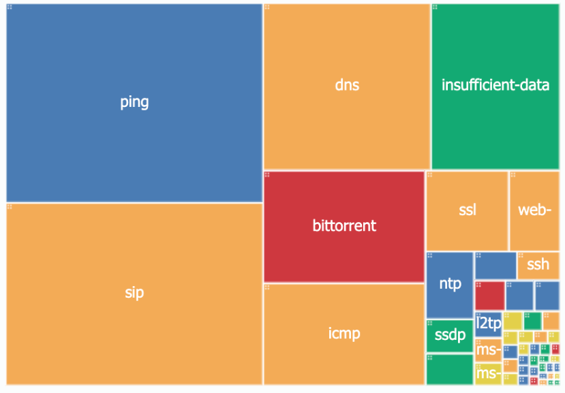
\includegraphics[width=0.6\linewidth]{用户应用类型图.png}
  \caption{用户应用类型图}
  \label{fig:用户应用类型图}
\end{figure}
% 接下来我们将以校园网为例,进行异常检测算法和系统的研究。清华大学校园网是全球规模最大,架构最复杂,流量场景最多变的校园网之一,具有以下几个特点:
% 1.	用户规模大,流量峰值高。每天有10万台设备活跃在线,同时在线设备最多为7万台,峰值流量约为30Gbps/s.
% 2.	用户应用类型多,远比一般的企业网复杂,在网络环境中几百种应用同时使用,这给数据分析带来了很多困难。
% 3.	异常流量是常态。扫描流量、攻击流量占比多。
% 这些特点给异常检测的研究和实现带来了诸多挑战。

% \section{研究内容}
% 围绕1.1节中提到的清华大学校园网流量异常检测的特点和挑战,本文分别展开了以下三方面研究:首先分析对比了开源数据集与


\section{论文的研究内容}
围绕1.1节中提到的清华大学校园网流量异常检测的特点和挑战,本文分别展开了以下三方面的研究:
\begin{enumerate}
  \item 本文分析对比了流量异常检测领域的两个经典开源数据集UNSW-NB15和CICIDS2017,引入了清华大学校园网的真实数据集,并且分别在这几个数据集上对现有的异常检测算法进行了实验对比。
    \item 在现有算法的基础上,本文将特征关系引入到神经网络的训练中,提出了一种基于特征之间关系图的循环神经网络算法(FG-RNN,Feature Graph-Recurrent Neural Network)。在复杂的网络流量环境下,流量特征种类繁多,且特征之间的相关性会随着流量变化而变化。原有的异常检测算法通常直接利用提取的特征进行训练,本文提出的FG-RNN算法有效利用了特征之间的相关性信息,将其加入到神经网络的训练过程中。
    \item 本文对基于特征之间关系图的循环神经网络算法进行了流式改造,使之能够满足当前实时异常检测的需求。为了应对海量的校园网流量数据和高速数据流,本文设计了一个基于spark streaming的实时异常检测系统。该系统分为输入模块、模型模块、检测模块三部分,输入模块负责将流量数据进行窗口划分、特征选择、特征抽取、合并计算,得到的特征矩阵与预训练得到的关系矩阵一同送到模型中进行训练,模型中的参数每2小时更新一次,最后由检测模块对当前流量进行判别,并给出异常流量的类别。

\end{enumerate}

\section{论文内容和组织结构}
第一章为引言,主要介绍本文的研究背景以及本文的研究内容。

第二章是关于网络流量异常检测的相关工作综述。首先对网络流量异常的定义和分类进行了介绍;接下来着重介绍了基于不同原理的异常检测算法;然后在开源数据集上对部分经典算法进行了复现,对比了其优缺点;最后,指出了现有的异常检测算法在当前大规模流量环境下存在的主要问题。

第三章至第五章是本文的主要研究内容。第三章分析对比了开源数据集与校园网真实数据集,并且在多个数据集上对现有的算法进行了实验对比。第四章提出了基于特征关系图的循环神经网络算法,并进行了算法性能评估。第五章设计并实现了一个基于spark streaming的流式处理系统。

最后,第六章对全文进行了总结,并且提出了未来展望。
